\documentclass[aspectratio=169]{beamer}

\graphicspath{{figures/}}

% Document metadata
\title{TIS18755P \\ Internet of Thing}
\subtitle{Catatan Kuliah \#1}
\author[AMH]{Alauddin Maulana Hirzan, M. Kom}
\institute{Universitas Semarang}
\date{}

% Image for the title page (use includegraphics option to properly size/place it)
\titlegraphic{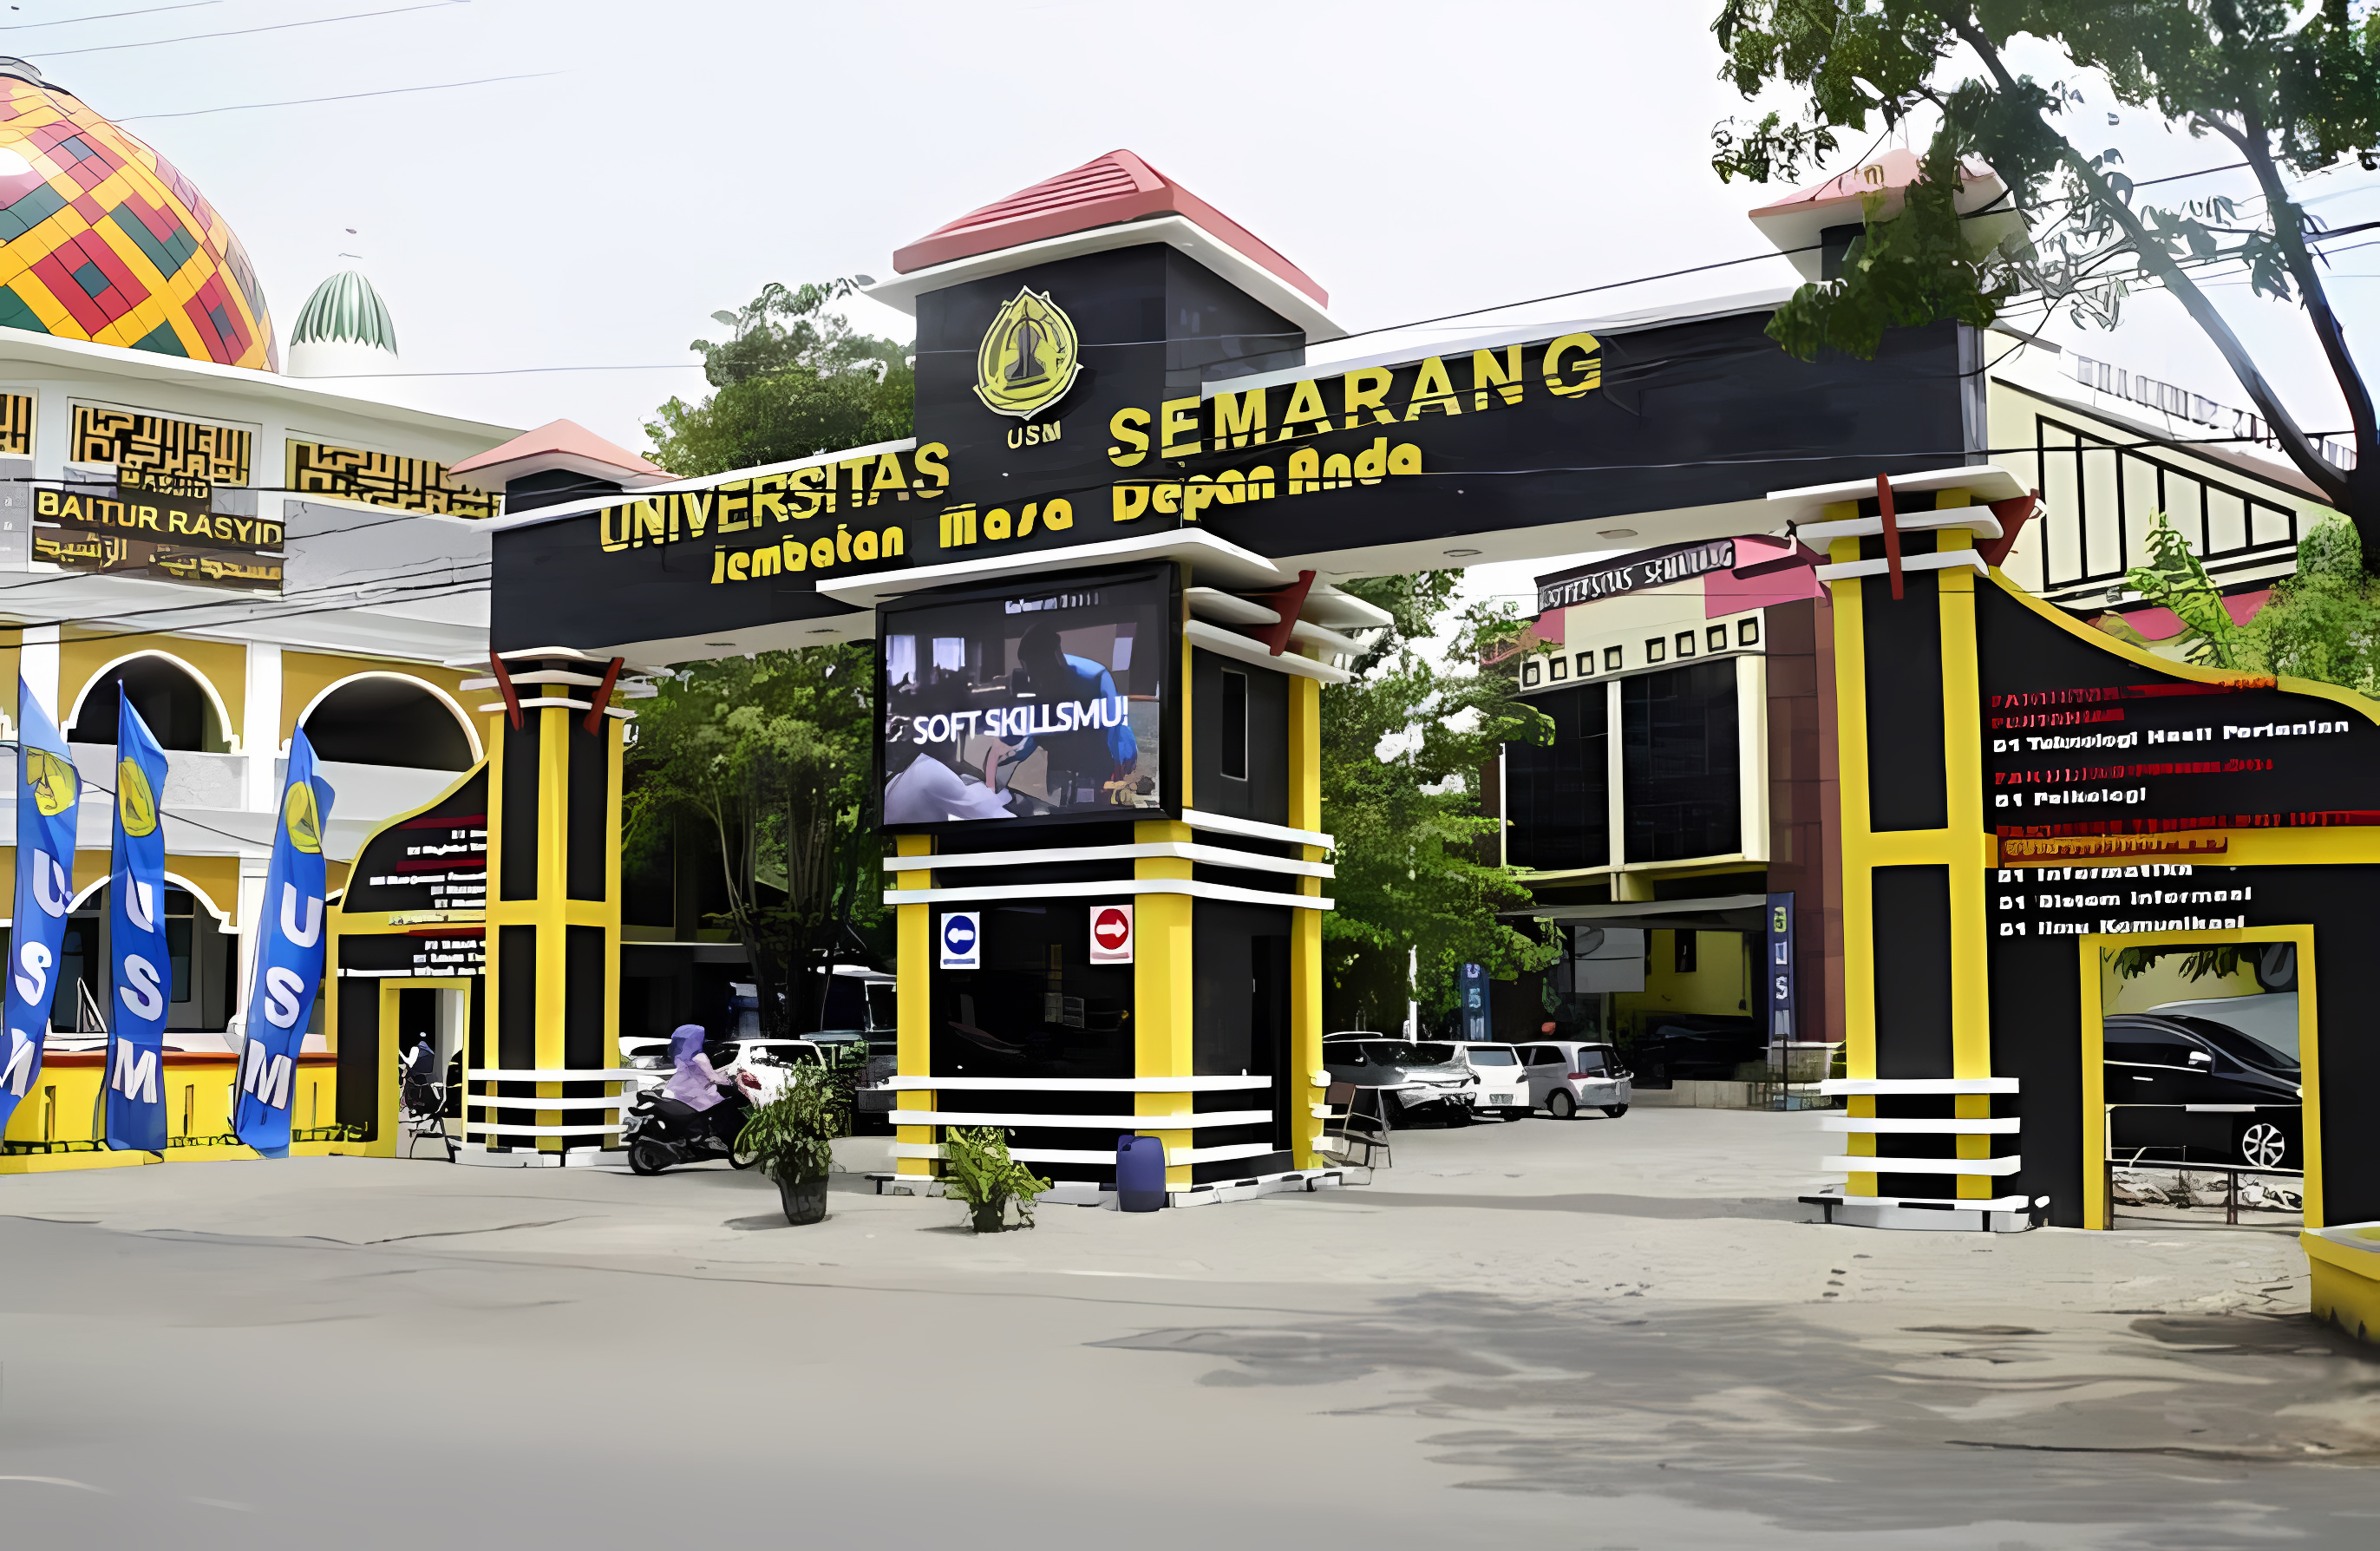
\includegraphics[height=\paperheight]{background.jpg}}

\usetheme[sectionstyle=style2]{trigon}

% Define logos to use (comment if no logo)
\smalllogo{logo_usm} % Used on top right corner of regular frames
% ------ If you want to change the theme default colors, do it here ------
\definecolor{tPrim}{HTML}{FF0000}   % Green
\definecolor{tSec}{HTML}{289B38}    % Green light
\definecolor{tAccent}{HTML}{F07F3C} % Orange

% ------ Packages and definitions used for this demo. Can be removed ------
\usepackage{appendixnumberbeamer} % To use \appendix command
\pdfstringdefDisableCommands{% Fix hyperref translate warning with \appendix
\def\translate#1{#1}%
}
\usepackage{pgf-pie} % For pie charts
\usepackage{caption} % For subfigures
\usepackage{subcaption} % For subfigures
\usepackage{xspace}
\usepackage{multicol}
\usepackage{ragged2e}
\newcommand{\themename}{\textbf{\textsc{trigon}}\xspace}
\usepackage[scale=2]{ccicons} % Icons for CC-BY-SA
\usepackage{booktabs} % Better tables

%==============================================================================
%                               BEGIN DOCUMENT
%==============================================================================
\begin{document}

\titleframe

% Contoh Kode Slide
%\section{Introduction}
%\begin{frame}{\insertsectionhead}
%	\framesubtitle{A short introduction to Trigon}
%	\themename is a modern, elegant and versatile theme for Beamer, inspired by
%	the
%	\href{https://github.com/matze/mtheme}{\textsc{metropolis} theme} from Matthias
%	Vogelgesang.
%	\vfill
%	\themename comes with lots of nice extra features
%	\begin{itemize}
%		\item Multiple style variations for title, section and normal slides
%		\item Simple customization of theme colors
%		\item Lots of convenient options to tweak the design
%	\end{itemize}
%\end{frame}

% Contoh Kode Tabel
%  \begin{table}[H]
% \centering
% \caption{A nice table example}
% \begin{tabular}{@{} lccc @{}}
%    \toprule
%    & \textbf{Velocity} & \textbf{Angle}  & \textbf{Vertical force} \\
%    & $U$ & $\alpha$  & $F_z$ \\
%    & [m/s] & [$^\circ$]  & [N] \\
%    \midrule
%    2D simulation  & 9 & 2 & 9.23 \\
%    3D simulation  & 10.0 & 3 & 15.039 \\
%    Experiment A   & 11.31 & 2.5 & 13.2 \\
%    Experiment B   & 11.26 & 2.7 & 12.6 \\
%    Experiment C   & 11.33 & 2.47 & 13.6 \\
%    \bottomrule
%  \end{tabular}
%\end{table}

% Contoh Kode Gambar
%  \begin{figure}[ht!]
%	\begin{subfigure}[b]{0.3\textwidth}
%		\frame{\includegraphics[width=\textwidth]{layout_example-03.jpg}}
%		\caption*{plain}
%	\end{subfigure}
%	\hspace{\fill}
%	\begin{subfigure}[b]{0.3\textwidth}
%		\frame{\includegraphics[width=\textwidth]{layout_example-02.jpg}}
%		\caption*{style1}
%	\end{subfigure}
%	\hspace{\fill}
%	\begin{subfigure}[b]{0.3\textwidth}
%		\frame{\includegraphics[width=\textwidth]{layout_example-01.jpg}}
%		\caption*{style2 (default)}
%	\end{subfigure}
%\end{figure}

% Contoh Kode Blocks
% \begin{block}{Regular block}
%	Just a regular block
%\end{block}
%\begin{alertblock}{Alert block}
%	Some important thing
%\end{alertblock}
%\begin{exampleblock}{Example block}
%	No difference with regular block to avoid excessive distraction
%\end{exampleblock}

\setbeamertemplate{frame footer}{Alauddin Maulana Hirzan, M. Kom - Universitas Semarang}

\section{Komponen Internal IoT}

\begin{frame}{\insertsectionhead}
	\framesubtitle{Teknologi dibalik IoT}
	\justifying
	Perangkat \textit{Internet of Things} memiliki beberapa komponen dasar sebagai berikut:
	\begin{itemize}
		\item Papan PCB
		\item Arsitektur CPU / Mikrokontroler
		\item Interface
		\item Port
	\end{itemize}
	\vfill
	Komponen-komponen ini adalah komponen pembentuk papan IoT yang digunakan hingga saat ini.
\end{frame}

\begin{frame}{\insertsectionhead}
	\framesubtitle{\textit{The Board} \#1}
	\justifying
	Layaknya papan elektronik lainnya, perangkat \textit{Internet of Things} juga terdiri dari beberapa komponen elektronik seperti \textbf{resistor}, \textbf{kapasitor}, hingga \textbf{\textit{Integrated Circuit / IC}}. Namun yang membedakan teknologi ini dengan papan elektronik lainnya adalah \textbf{\textit{ukurannya}}
	\vfill
	Papan pemrosesan atau komputasi \textit{Internet of Things} memiliki ukuran hingga maksimal 3,5 inch secara diagonal. Sehingga komponen-komponen yang ada di dalamnya harus berukuran sangat-sangat kecil.
	\vfill
	Meski berukuran kecil, papan \textit{Internet of Things} juga sensitif terhadap \textit{Electric Static Discharge} / ESD atau dikenal sebagai listrik statis yang tersimpan di masing-masing komponen IoT.
\end{frame}

\begin{frame}{\insertsectionhead}
	\framesubtitle{\textit{The Board} \#2}
	\justifying
	\begin{block}{Peringatan}
		Korsleting bisa terjadi jika tangan basah atau benda metal menyentuh papan IoT yang baru dimatikan. ESD dapat terjadi meskipun perangkat IoT tidak pernah terhubung ke soket listrik.
	\end{block}
	\vfill
	Oleh karena itu, komponen-komponen IoT selalu dibungkus dalam plastik khusus agar terhindar dari ESD yang ada maupun debu-debu.
\end{frame}

\begin{frame}{\insertsectionhead}
	\framesubtitle{\textit{The Board} \#3}
	\justifying
	Papan IoT ini tentu saja memerlukan pasokan listrik untuk menghidupkan komponen lainnya. Sehingga dalam menyediakan daya untuk perangkat, pengguna harus memahami batasan pasokan listrik yang diterima oleh perangkat IoT.
	\vfill
	Standarnya perangkat IoT hanya boleh diberik listrik dengan tegangan 3.3V untuk papan berukuran kecil (Mikrokontroler) dan 5V papan berukuran 3.5\" (\textit{System-on-Chip}) tergantung dari manufaktur yang membuat.
\end{frame}

\begin{frame}{\insertsectionhead}
	\framesubtitle{\textit{The Board} \#4}
	\justifying
	\begin{block}{Peringatan - \textbf{\textit{Undervoltage}}}
		Perangkat yang diberi tegangan yang kurang dari standar akan menyebabkan perangkat mengalami \textit{Undervoltage}. Keadaan ini memaksa perangkat melakukan \textit{throttling} sehingga perangkat bekerja menjadi lambat, bahkan tidak akan menyala.
	\end{block}
	\vfill
	\begin{block}{Berbahaya - \textbf{\textit{Overvoltage}}}
		Kondisi ini sangat berbahaya bagi perangkat karena dapat menyebabkan kerusakan fatal pada perangkat. Meskipun beberapa perangkat sudah dilengkat dengan \textit{Overvoltage Protection}, namun fitur ini hanya berlaku sekali.
	\end{block}
\end{frame}

\begin{frame}{\insertsectionhead}
	\framesubtitle{\textit{The Board} \#4}
	\justifying
	\begin{figure}[ht!]
		\begin{subfigure}[b]{0.9\textwidth}
			\frame{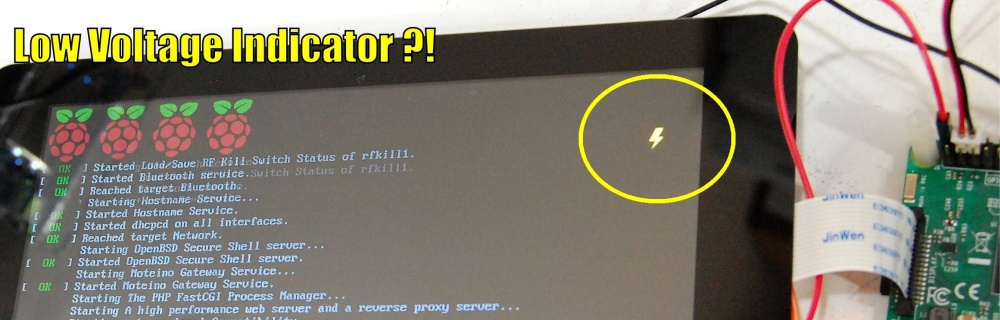
\includegraphics[width=\textwidth]{undervoltage-warning.jpg}}
			\caption*{Peringatan Voltase Rendah}
		\end{subfigure}
	\end{figure}
	\vfill
	Hal ini akan terjadi jika \textit{power supply} tidak sesuai atau komponen terlalu banyak
\end{frame}

\begin{frame}{\insertsectionhead}
	\framesubtitle{Skematik Raspberry Pi}
	\justifying
	\begin{figure}[ht!]
		\begin{subfigure}[b]{0.6\textwidth}
			\frame{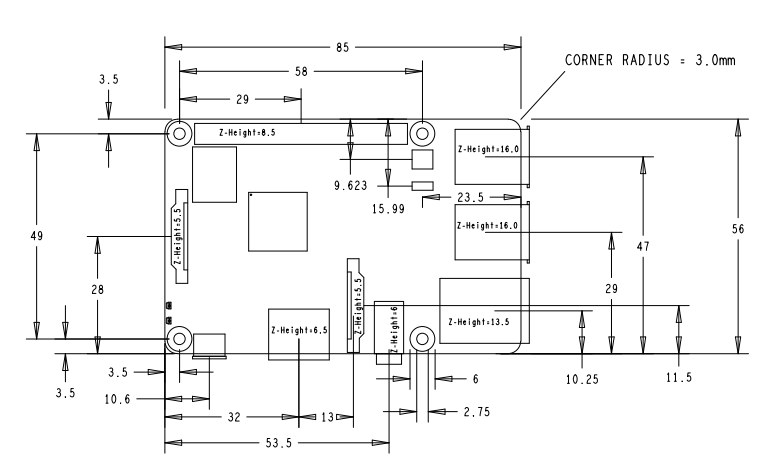
\includegraphics[width=\textwidth]{skematik-rpi.png}}
		\end{subfigure}
	\end{figure}
\end{frame}

\begin{frame}{\insertsectionhead}
	\framesubtitle{Skematik Arduino}
	\justifying
	\begin{figure}[ht!]
		\begin{subfigure}[b]{0.7\textwidth}
			\frame{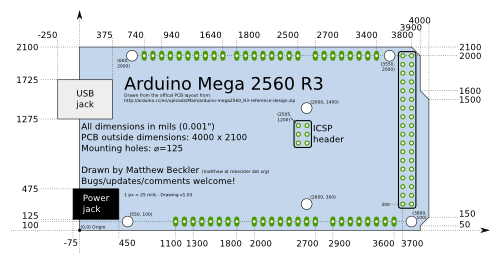
\includegraphics[width=\textwidth]{skematik-arduino.png}}
		\end{subfigure}
	\end{figure}
\end{frame}

\begin{frame}{\insertsectionhead}
	\framesubtitle{Arsitektur CPU}
	\justifying
	Dikarenakan penggunaan daya yang berbeda dengan komputer biasa, maka sebagian besar perangkat IoT dibuat dengan arsitektur CPU yang berbeda. Hal ini dikarenakan penggunaan daya yang rendah, sehingga prosesor biasa tidak bisa diguankan.
	\vfill
	Perangkat IoT biasanya menggunakan teknologi:
	\begin{itemize}
		\item Mikrokontroler
		\item System-on-Chip
	\end{itemize}
\end{frame}

\begin{frame}{\insertsectionhead}
	\framesubtitle{Mikrokontroler \#1}
	\justifying
	Mikrokontroler (kadang-kadang disebut MCU atau Unit Mikrokontroler) adalah Sirkuit Terpadu (IC) tunggal yang biasanya digunakan untuk aplikasi tertentu dan dirancang untuk mengimplementasikan tugas-tugas tertentu.
	\vfill
	Pada dasarnya, mikrokontroler mengumpulkan input, memproses informasi ini, dan mengeluarkan tindakan tertentu berdasarkan informasi yang dikumpulkan. Mikrokontroler biasanya beroperasi pada kecepatan yang lebih rendah, sekitar kisaran 1MHz hingga 200 MHz, dan perlu dirancang untuk mengkonsumsi lebih sedikit daya
\end{frame}

\begin{frame}{\insertsectionhead}
	\framesubtitle{Mikrokontroler \#2}
	\justifying
	Mikrokontroler dapat dilihat sebagai komputer kecil, karena komponen penting di dalamnya; Central Processing Unit (CPU), Random-Access Memory (RAM), Flash Memory, Serial Bus Interface, Input/Output Ports (I/O Ports).
	\vfill
	\begin{block}{Info}
		Dikarenakan ukurannya yang kecil dan murah, perangkat IoT berbasis mikrokontroler dibanderol lebih murah dibandingkan berbasis \textit{System-on-Chip}. Namun memiliki kelemahan dalam kekuatan komputasi
	\end{block}
\end{frame}

\begin{frame}{\insertsectionhead}
	\framesubtitle{Isi Mikrokontroler}
	\justifying
	\begin{figure}[ht!]
		\begin{subfigure}[b]{0.5\textwidth}
			\frame{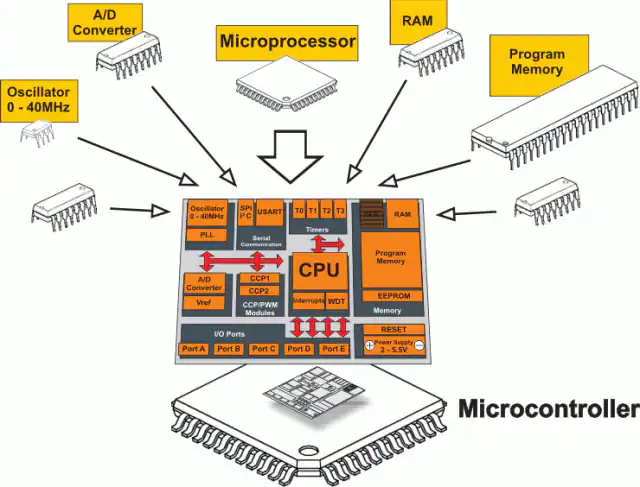
\includegraphics[width=\textwidth]{mikrokontroler.png}}
		\end{subfigure}
	\end{figure}
\end{frame}

\begin{frame}{\insertsectionhead}
	\framesubtitle{Desain Mikrokontroler}
	\justifying
	Dua komponen utamanya adalah Unit Logika Aritmatika (ALU), yang melakukan operasi aritmatika dan logika, dan Unit Kontrol (CU), yang menangani semua eksekusi instruksi prosesor.
	\vfill
	\begin{figure}[ht!]
		\begin{subfigure}[b]{0.7\textwidth}
			\frame{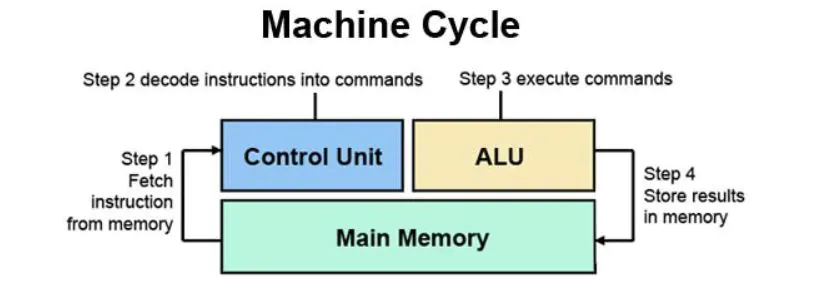
\includegraphics[width=\textwidth]{siklus-kontroler.png}}
		\end{subfigure}
	\end{figure}
\end{frame}

\begin{frame}{\insertsectionhead}
	\framesubtitle{Arduino dengan \textit{ATMega}}
	\justifying
	\begin{figure}[ht!]
		\begin{subfigure}[b]{0.5\textwidth}
			\frame{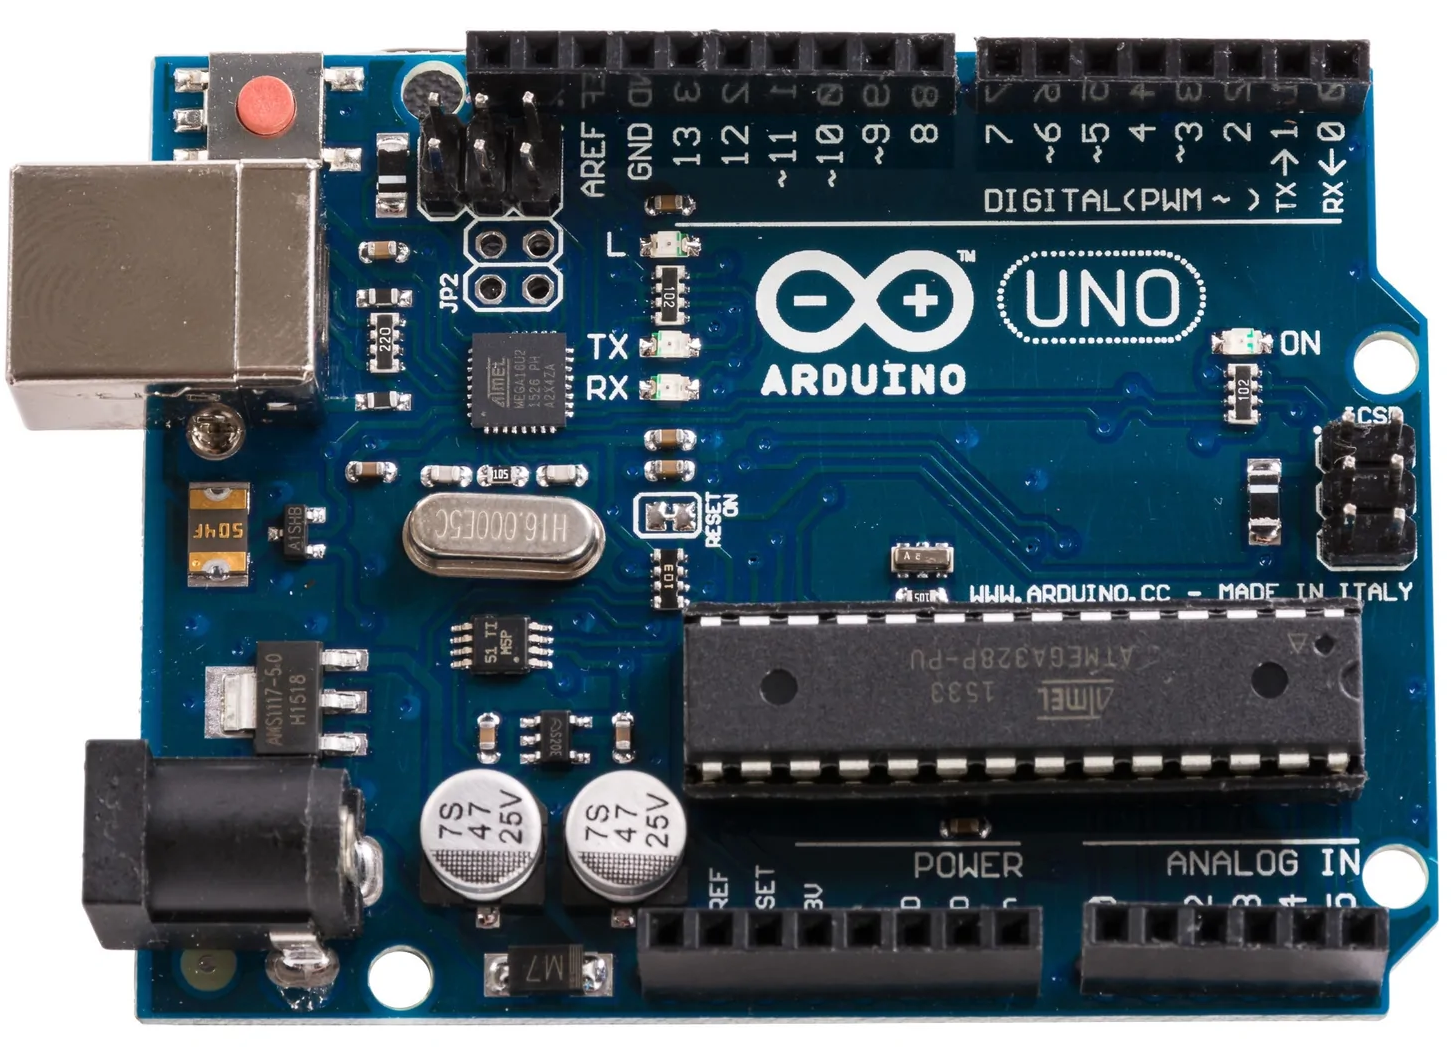
\includegraphics[width=\textwidth]{atmega.png}}
		\end{subfigure}
	\end{figure}
\end{frame}

\begin{frame}{\insertsectionhead}
	\framesubtitle{\textit{System-on-Chip} \#1}
	\justifying
	\textit{System-on-Chip}, adalah sirkuit terpadu yang mengintegrasikan semua atau sebagian besar komponen komputer atau sistem elektronik lainnya. Komponen ini hampir selalu mencakup unit pemrosesan pusat (CPU), antarmuka memori, perangkat input/output, antarmuka input/output, dan antarmuka penyimpanan sekunder, sering kali bersama dengan komponen lain seperti modem radio dan unit pemrosesan grafis (GPU). – semua dalam satu substrat atau microchip.
\end{frame}

\begin{frame}{\insertsectionhead}
	\framesubtitle{Isi \textit{System-on-Chip}}
	\justifying
	\begin{figure}[ht!]
		\begin{subfigure}[b]{0.65\textwidth}
			\frame{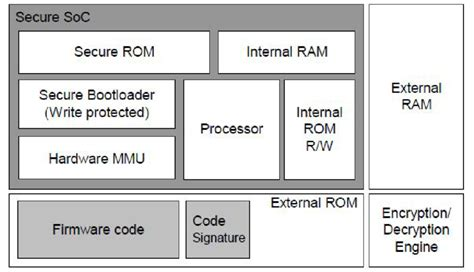
\includegraphics[width=\textwidth]{komponen-soc.jpg}}
		\end{subfigure}
	\end{figure}
\end{frame}

\begin{frame}{\insertsectionhead}
	\framesubtitle{Isi \textit{System-on-Chip}}
	\justifying
	Meski hampir memiliki fitur seperti komputer biasa, namun SoC lebih lengkap dengan komponen seperti berikut:
	\vfill
	\begin{itemize}
		\item Processor cores
		\item Memory
		\item Interfaces
		\item Digital signal processors
		\item GPU
		\item Network on a chip
	\end{itemize}
\end{frame}

\begin{frame}{\insertsectionhead}
	\framesubtitle{Raspberry Pi 2 dengan Broadcom SoC}
	\justifying
	\begin{figure}[ht!]
		\begin{subfigure}[b]{0.5\textwidth}
			\frame{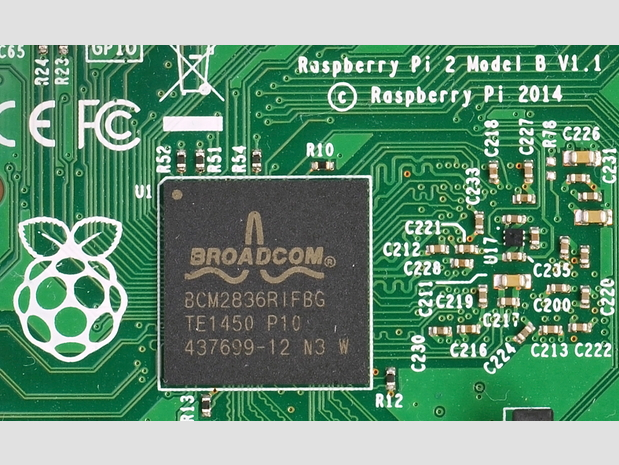
\includegraphics[width=\textwidth]{bcm.jpg}}
		\end{subfigure}
	\end{figure}
\end{frame}

\begin{frame}{\insertsectionhead}
	\framesubtitle{\textit{Advanced RISC Machine}}
	\justifying
	Beberapa \textit{System-on-Chip} menggunakan teknologi \textit{Advanced RISC Machine} sebagai arsitektur CPU.  Teknologi ini sangat berbeda dengan yang dihadirkan oleh Intel maupun AMD yang menggunakan teknologi CISC.
	\vfill
	\begin{figure}[ht!]
		\begin{subfigure}[b]{0.5\textwidth}
			\frame{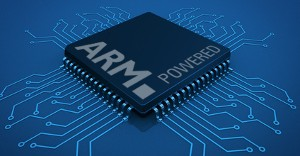
\includegraphics[width=\textwidth]{arm.jpg}}
		\end{subfigure}
	\end{figure}
\end{frame}

\begin{frame}{\insertsectionhead}
	\framesubtitle{Antarmuka \textit{Internet of Things}}
	\justifying
	Antarmuka ini merujuk ke protokol komunikasi secara fisik, bukan melalui jaringan. Dikarenakan perangkat \textit{Internet of Things} juga harus berkomunikasi dengan sensor maupun aktuator sehingga antarmuka komunikasi media fisik ini tersedia untuk digunakan.
	\vfill
	Jenis komunikasi protokol yang bisa digunakan:
	\begin{itemize}
		\item UART
		\item I2C
		\item SPI
		\item GPIO
	\end{itemize}
\end{frame}

\begin{frame}{\insertsectionhead}
	\framesubtitle{UART dan I2C}
	\justifying
	UART (\textit{Universal Asynchronous Receiver / Transmitter}) adalah implementasi perangkat keras yang mendukung komunikasi serial dua arah, asinkron.
	\vfill
	I2C (\textit{Inter-Integrated Circuit}) adalah antarmuka komunikasi serial dua arah, sinkron. Jika beroperasi pada dua saluran dalam mode setengah dupleks.
		\begin{figure}[ht!]
		\begin{subfigure}[b]{0.25\textwidth}
			\frame{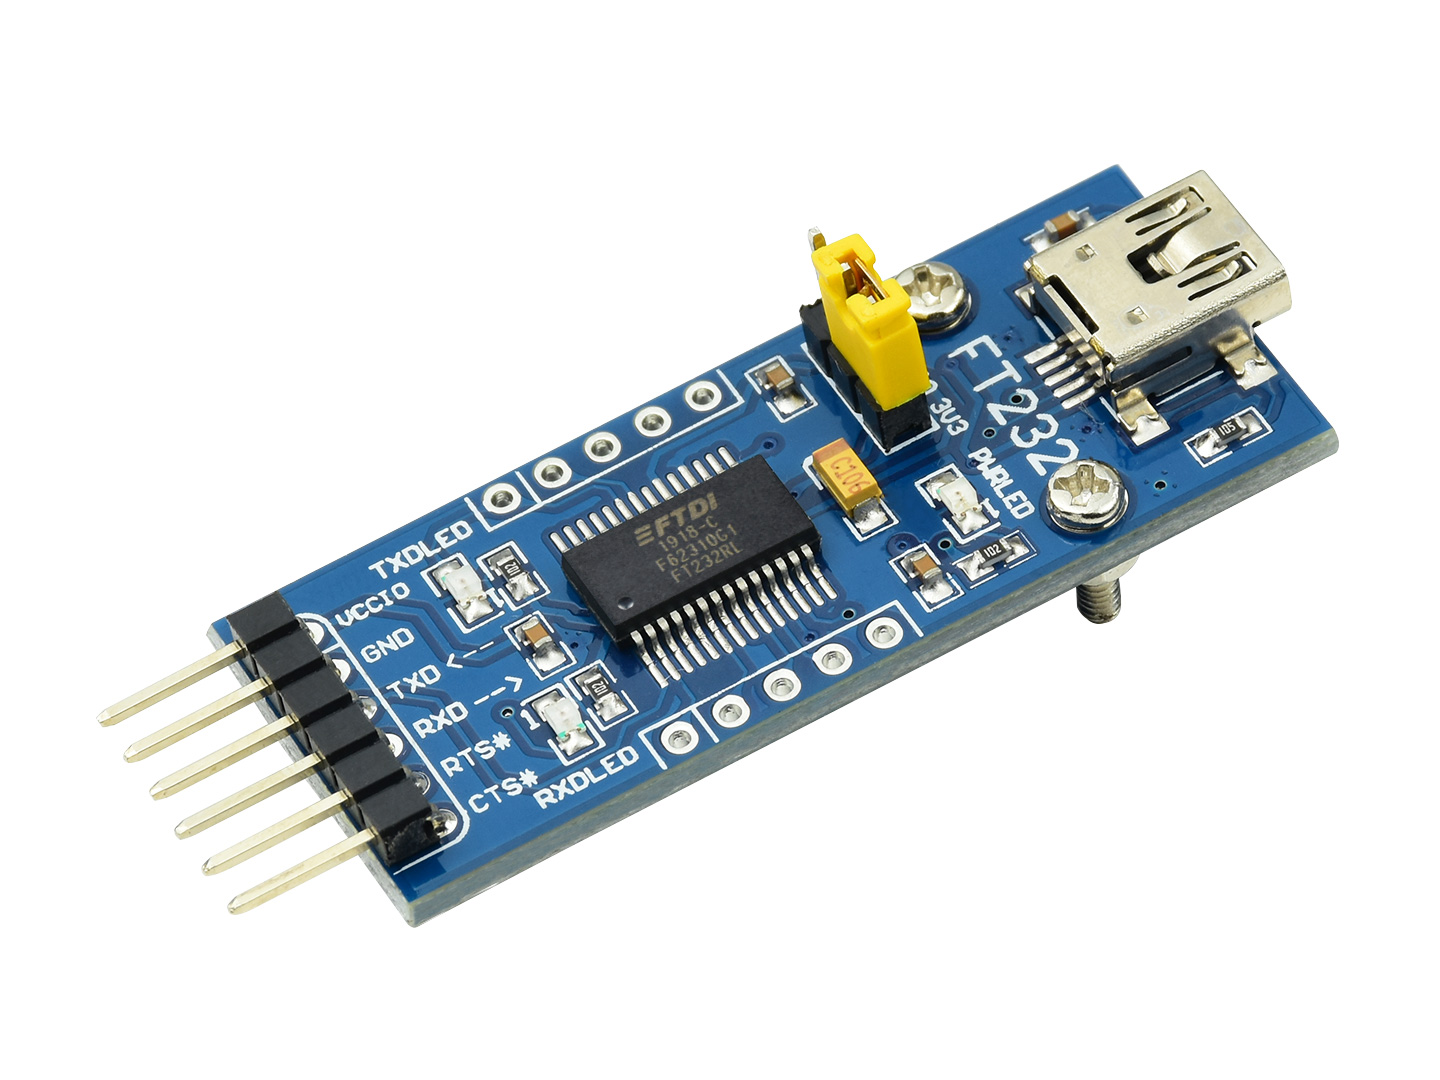
\includegraphics[width=\textwidth]{uart.jpg}}
			\caption*{Komponen UART}
		\end{subfigure}
		\hspace{50pt}
		\begin{subfigure}[b]{0.25\textwidth}
			\frame{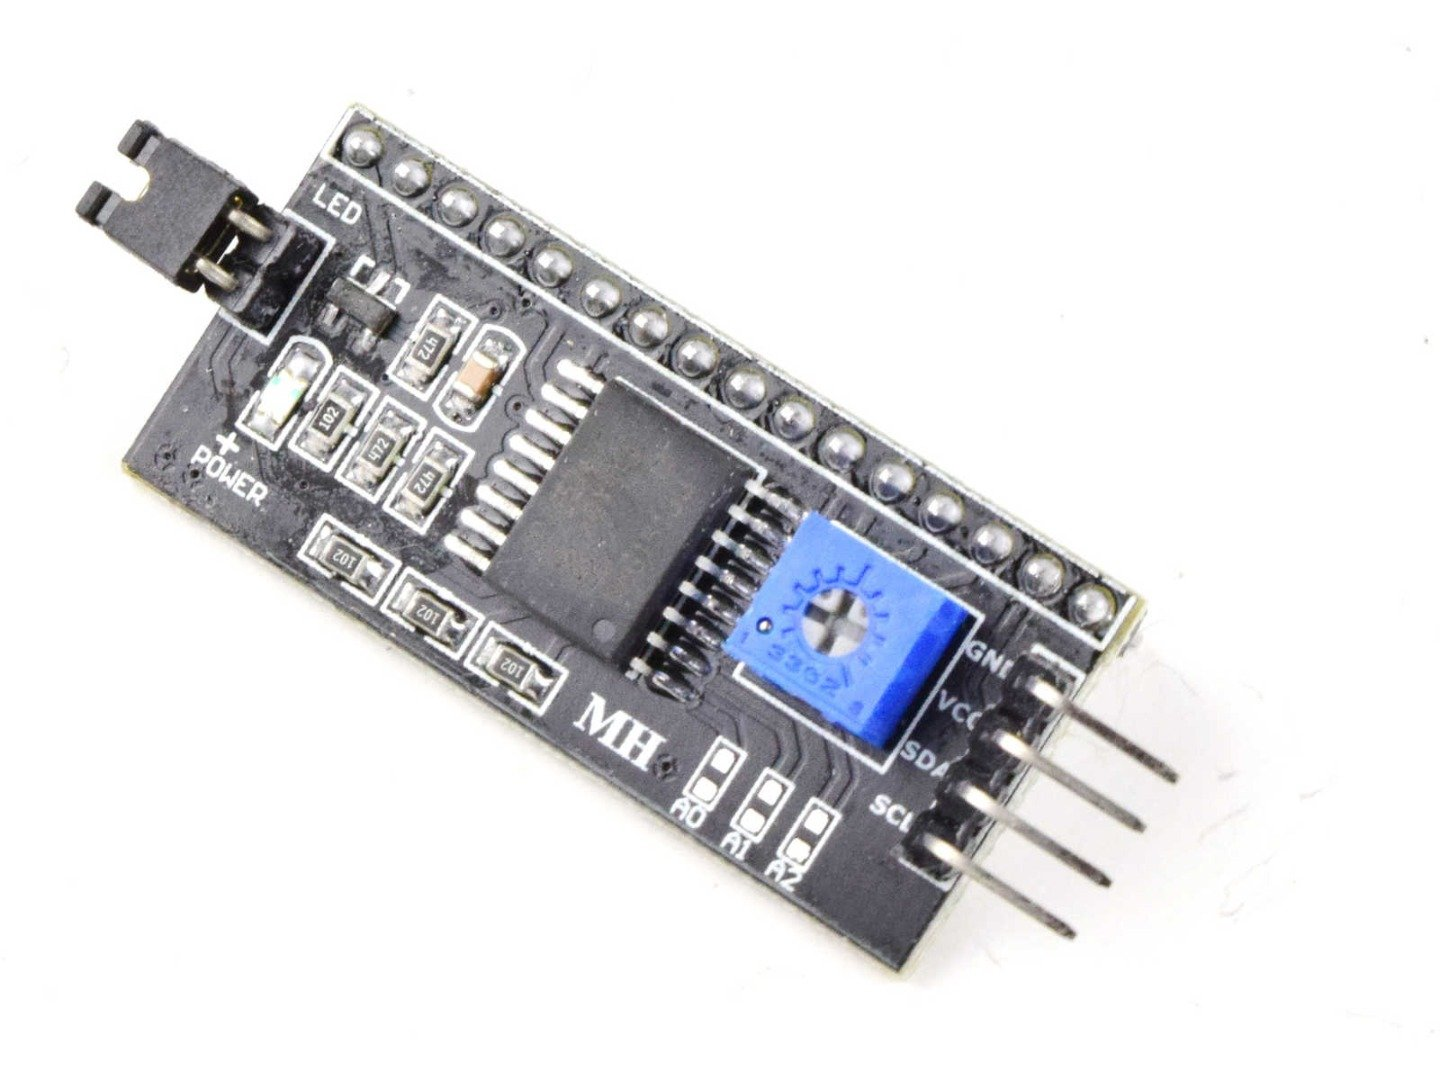
\includegraphics[width=\textwidth]{i2c.jpg}}
			\caption*{Komponen I2C}
		\end{subfigure}
	\end{figure}
\end{frame}

\begin{frame}{\insertsectionhead}
	\framesubtitle{SPI dan GPIO}
	\justifying
	SPI (\textit{Serial Peripheral Interface}) adalah antarmuka komunikasi serial dua arah, sinkron, - seperti I2C. Namun tidak seperti I2C, SPI beroperasi pada full duplex, artinya data dapat dikirim dan diterima secara bersamaan.
	\vfill
	GPIO (\textit{General-purpose Input/Output})adalah pin sinyal pada sirkuit atau papan terintegrasi yang dapat digunakan untuk melakukan fungsi input atau output digital. Secara desain, ia tidak memiliki tujuan yang telah ditentukan sebelumnya dan dapat digunakan oleh pengembang perangkat keras atau perangkat lunak untuk melakukan fungsi yang mereka pilih.
\end{frame}

\begin{frame}{\insertsectionhead}
	\framesubtitle{UART dan I2C}
	\justifying
	\begin{figure}[ht!]
		\begin{subfigure}[b]{0.25\textwidth}
			\frame{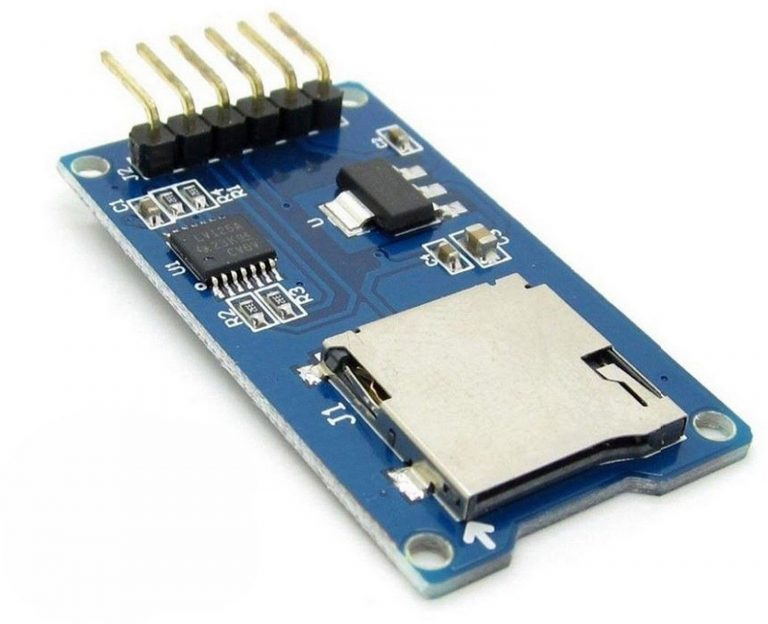
\includegraphics[width=\textwidth]{spi.jpg}}
			\caption*{Komponen UART}
		\end{subfigure}
		\hspace{50pt}
		\begin{subfigure}[b]{0.25\textwidth}
			\frame{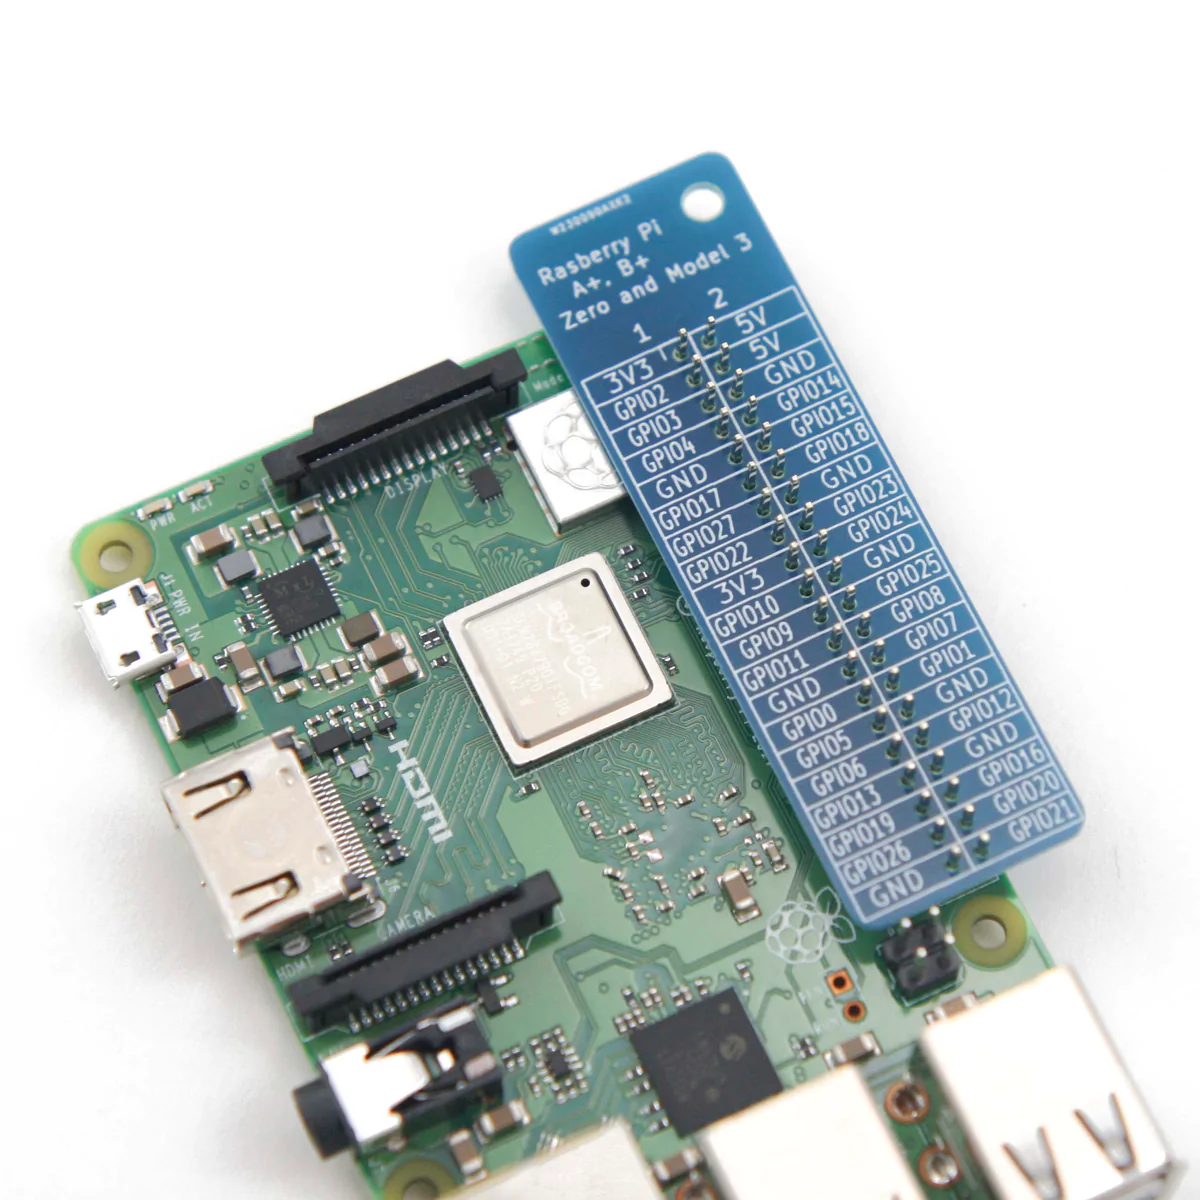
\includegraphics[width=\textwidth]{gpio.png}}
			\caption*{Komponen I2C}
		\end{subfigure}
	\end{figure}
\end{frame}

\begin{frame}{\insertsectionhead}
	\framesubtitle{\textit{I/O Ports}}
	\justifying
	Port I/O adalah apa yang digunakan mikrokontroler untuk terhubung ke aplikasi dunia nyata. Input menerima perubahan di dunia nyata, dari penginderaan, hingga tombol tekan, dan banyak lagi.
	\vfill
	\begin{figure}[ht!]
		\begin{subfigure}[b]{0.4\textwidth}
			\frame{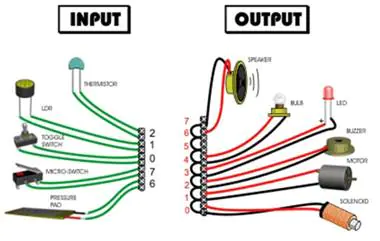
\includegraphics[width=\textwidth]{io-kontroler.png}}
		\end{subfigure}
	\end{figure}
\end{frame}

\setbeamertemplate{background} 
{
	\includegraphics[width=\paperwidth,height=\paperheight]{thank-you.jpg}
}
\begin{frame}[plain]
\end{frame}

\end{document}
